\chapter{Design and Implementation}
\label{chap:design_and_implementation}


\section{Introduction}
In this chapter, we will discuss the design and implementation of the \ac{POP} algorithm.
We will start by discussing the design of the algorithm,
and then we will discuss the implementation of the algorithm in C\#.

\section{Design of the Algorithm}
\subsection{Nondeterministic Achievers \& Threat Search} \label {subsec:nondeterministic_achievers_threat_search}
\acf{POP} needs to be able to handle some form of nondeterminism in the planning domain. This is because the planner needs
to be able to handle situations where there are multiple ways to achieve a precondition
of an action. Nondeterminism is a concept that is used in computer science to describe the occurrence of events without a predictable outcome, where multiple outcomes are possible from a given state. In the context of planning, nondeterminism is used to describe the situation where there are multiple ways to achieve a precondition of an action, for example.
This cannot be achieved in practice without trying to search all possible ways of the choices that can be made.
So, to model nondeterminism in the planning domain, we need to use some form of graph search algorithm to search for all possible ways to achieve a precondition of an action efficiently. In this project, multiple graph search algorithms were implemented to handle nondeterminism in the planning domain. These algorithms are \ac{A*} Search, \ac{BFS}, and \ac{DLS} which is a variation of \ac{DFS}. All of these algorithms are discussed in detail in the following sections.


\subsection{Graph Search Algorithms} \label{subsec:graph_search_algorithms}
Graph search algorithms are widely used in computer science to solve problems that can be represented as graphs. They have many applications in various fields such as artificial intelligence, computer graphics, and computer vision. In this project, graph search algorithms were used to solve the problem of nondeterminism in the planning domain.
\subsubsection{\acf{A*} Search Algorithm} \label{subsubsec:a_star}
\ac{A*} Search is a graph search \& traversal algorithm that is widely used in computer science due to its efficiency, optimality, and completeness. It is an informed search algorithm that uses a heuristic function to estimate the cost of reaching the goal from a given state. The heuristic function is used to guide the search towards the goal state by selecting the most promising nodes to explore. \ac{A*} Search is an extension of Dijkstra's algorithm that uses a heuristic function to estimate the cost of reaching the goal from a given state. \ac{A*} is a Best First Search algorithm that uses a priority queue to store the nodes to be explored. The priority queue is ordered based on a cost function that combines the cost of reaching the node from the start state and the heuristic estimate of the cost of reaching the goal from the node. The cost function is defined as $f(n) = g(n) + h(n)$, where $g(n)$ is the cost of reaching the node from the start state and $h(n)$ is the heuristic estimate of the cost of reaching the goal from the node. The algorithm selects the node with the lowest $f$ value from the priority queue and explores its neighbors until the goal is reached. The algorithm is guaranteed to find the optimal solution if the heuristic function is admissible, i.e., it never overestimates the cost of reaching the goal from a given state. The algorithm is also complete if the search space is finite and the heuristic function is consistent.

In this project, $g(n)$ is the path (level) cost from the root node to the current node, and $h(n)$ heuristic was chosen to be the number of unsatisfied preconditions, i.e., the count of pairs in the $agenda$ discussed in section {\ref{subsec:pop_algorithm}}.

\subsubsection{\acf{DLS} Search Algorithm} \label{subsubsec:dls}
First, let's discuss the \ac{DFS} algorithm.
\ac{DFS} is an uninformed search algorithm that is widely used in computer science to explore a graph or tree data structure. It is a depth-first traversal algorithm that explores the nodes deep in the graph before exploring the nodes at the same level. The algorithm starts at the root node and explores the nodes along each branch before backtracking to explore the other branches. The algorithm uses a stack data structure to store the nodes to be explored. The algorithm is not guaranteed to find the optimal solution, but it is complete if the search space is finite. The algorithm is also efficient in terms of memory usage as it only needs to store the nodes along the current path. However, the algorithm can get stuck in infinite loops if the graph contains an infinite deep path. To avoid this problem, a depth limit can be imposed on the search to limit the depth of the search tree. This is known as the \acf{DLS} algorithm. The algorithm is similar to \ac{DFS} but with an additional depth limit parameter that specifies the maximum depth of the search tree. The algorithm stops exploring a branch when the depth limit is reached and backtracks to explore other branches. The algorithm is complete if the depth limit is greater than the depth of the optimal solution. The algorithm is also efficient in terms of memory usage. In this project, \ac{DLS} was also provided as an option to be used in the \ac{POP} algorithm.

\subsubsection{\acf{BFS} Search Algorithm} \label{subsubsec:bfs}
\ac{BFS} is an uninformed search algorithm that is widely used to explore a graph or tree data structure. It is a breadth-first traversal algorithm, meaning that it explores the nodes at the same level before exploring the nodes at the next level. The algorithm starts at the root node and explores the nodes at the same level before moving to the next level. The algorithm uses a queue data structure to store the nodes to be explored. The algorithm is guaranteed to find a solution if one exist, even if the graph is infinite. However, the algorithm is not guaranteed to always find the optimal solution. The algorithm is also inefficient in terms of memory usage as it needs to store all the nodes at the current level. In this project, \ac{BFS} was also provided as an option to be used in the \ac{POP} algorithm.

\subsection{Unification Algorithm} \label{subsec:unification_algorithm}
Finding the \acf{MGU} of two terms is a crucial step in the \ac{POP} algorithm. The \ac{MGU} is used to unify two terms by finding a substitution that makes the two terms equal. The \ac{MGU} is the most general substitution that can be applied to the two terms to make them equal. The \ac{MGU} is used to unify the preconditions of an action with the current state of the world to determine if the action can be applied. The \ac{MGU} is also used to unify the effects of an action that can be used, for example, to detect threats in the partial plan. In this project, the \ac{MGU} algorithm was implemented using a variation of the unification algorithm discussed in Russell and Norvig's book \cite{RN2020_Ch.9}.
The algorithm is described as follows:
% \begin{algorithm}
%     \caption{Unification Algorithm}
%     \begin{algorithmic}
%         \STATE \textbf{function} UNIFY($x, y, \theta$)
%         \IF{$\theta = \text{failure}$}
%         \RETURN failure
%         \ELSIF{$x = y$}
%         \RETURN $\theta$
%         \ELSIF{$\text{VARIABLE?}(x)$}
%         \RETURN UNIFY-VAR($x, y, \theta$)
%         \ELSIF{$\text{VARIABLE?}(y)$}
%         \RETURN UNIFY-VAR($y, x, \theta$)
%         \ELSIF{$\text{COMPOUND?}(x) \land \text{COMPOUND?}(y)$}
%         \RETURN UNIFY($\text{ARGS}(x), \text{ARGS}(y), \text{UNIFY}(\text{OP}(x), \text{OP}(y), \theta)$)
%         \ELSE
%         \RETURN failure
%         \ENDIF
%     \end{algorithmic}
% \end{algorithm}



% image of the pop class diagram (POP.png)
\begin{figure}[ht]
    \centering
    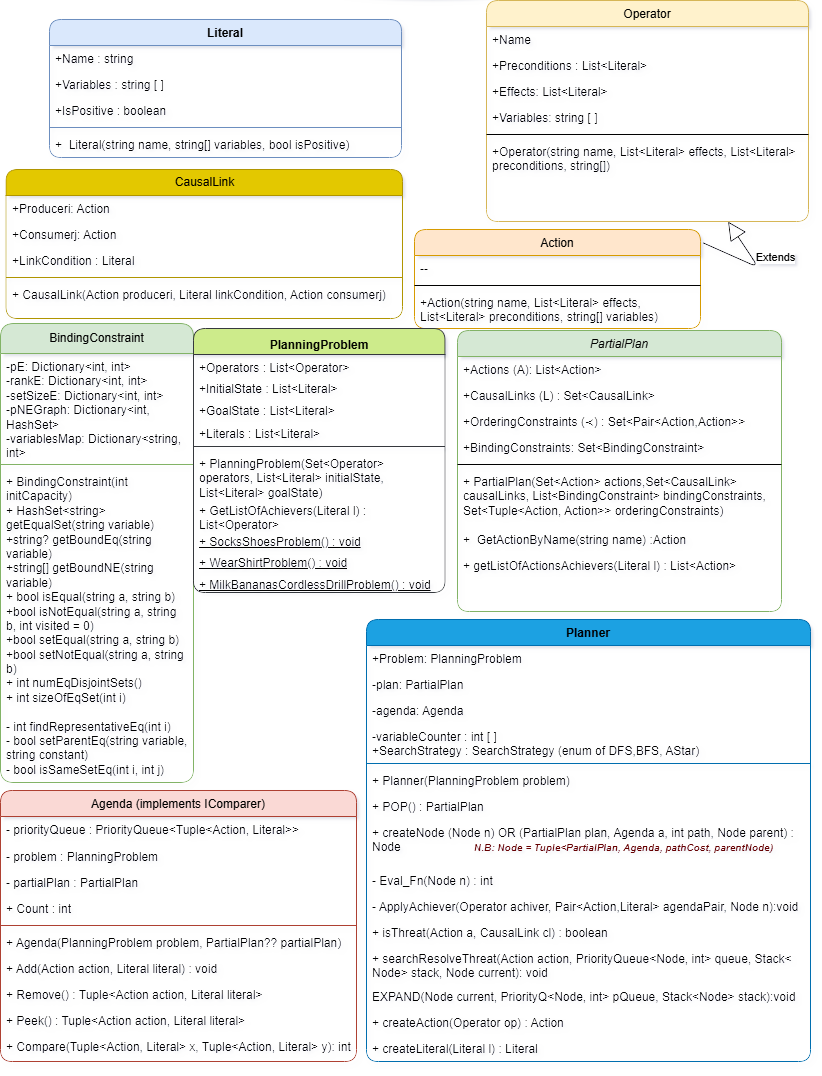
\includegraphics[width=0.9\textwidth]{images/POP.png}
    \caption[Class Diagram of the POP Algorithm]{Class Diagram of the POP Algorithm}
    \label{fig:pop}
\end{figure}